\documentclass{wustlthesis}

% Custom fonts
\setmainfont{SourceSerif4}[
    Path=./fonts/source-serif/,
    Ligatures=TeX,
    UprightFont=*-Regular, ItalicFont=*-It,
    BoldFont=*-Bold, BoldItalicFont=*-BoldIt
]
\setsansfont{SourceSans3}[
    Path=./fonts/source-sans/,
    Ligatures=TeX,
    UprightFont=*-Regular, ItalicFont=*-It,
    BoldFont=*-Bold, BoldItalicFont=*-BoldIt
]
\setmathfont{STIXTwoMath}[math-style=ISO]

% Re-calculate the lengths of a text line using the current font
\setlxvchars[\normalfont\normalsize]
\setxlvchars[\normalfont\normalsize]
\checkandfixthelayout[classic]

% Enable refinements of typographics
\usepackage[
    activate=true,
    disable=false,  % enable microtype even in the draft mode
    babel=true,     % enable language-specific kerning.
]{microtype}
% Tweak Source Serif font like Times
% \DeclareMicrotypeAlias{SourceSerif4}{ptm}

% Tweak LaTeX line breaking
\midsloppy

% Hyperlinks
\usepackage{hyperref}
\hypersetup{%
    colorlinks=true,
    linkcolor=black,
    urlcolor=[rgb]{0.0855,0.3675,0.5470},
    citecolor=black%
}
% default URL style
\urlstyle{same}

% Tables
\usepackage{threeparttable}
\usepackage{multirow}  % allow multiple lines in a table cell

% Graphics
\usepackage{graphicx}

% Subcaptions
% The caption format is "Figure 1. Main. (A) xxx. (B) yyy".
% And the label reference format is "Figure 1A".
\usepackage{subcaption}
\renewcommand\thesubfigure{\Alph{subfigure}}
\renewcommand\thesubtable{\Alph{subtable}}
\captionsetup{subrefformat=parens}

% Allowing subcaptions when all figure panels are combined
% into one source image. Based on https://tex.stackexchange.com/a/255790
\newcommand{\phantomlabel}[1]{%
    \parbox{0pt}{\phantomsubcaption\label{#1}}%
}

% Add a note for figure caption spanning multiple pages
\newcommand{\legendcontdnote}{%
    \footnotesize\itshape%
    \sourceatright[2em]{(legend continued on next page)}%
}
\newcommand{\legendcontdref}[1]{%
    \emph{(\fref{#1} continued)}%
}

% Bibliography
\usepackage[
    backend=biber,
    style=nature,
    date=year,
    isbn=false, url=false, doi=true,
    minnames=1, maxnames=9,
    backref=true,
    % block=space,   % allow additional horizontal space between blocks
]{biblatex}
% rename bibliography section name
\DefineBibliographyStrings{english}{
    bibliography = {References},
    backrefpage = {cited on p\adddot},
    backrefpages = {cited on pp\adddot}}
% hide PubMed ID (pmid:xxx) in the bibliography
\DeclareFieldFormat{eprint:pmid}{}

% define the bibliography path
\addbibresource{references.bib}

% Helper commands
\newcommand{\gene}[1]{\textit{#1}}

% Configure title page
\settitle{%
    Building a toolbox and insights toward\\
    proteogenomic characterization of glioblastoma%
}
\setauthor{Liang-Bo Wang}
\setthesistype{Dissertation}
\setthesisdegree{Doctor of Philosophy}
\setthesisdegreeabbrv{Ph.D.}
% Degree officially earn date must be in December, May, or August
\setdegreedatemy{December}{2021}
\setthesisadvisorwithtitle{Professor Li Ding, Chair}
\setthesiscommittee{%
    Li Ding, Chair\\
    Joshua B. Rubin\\
    Stephen T. Oh\\
    John R. Edwards\\
    Milan G. Chheda%
}
\setthesisschool{Division of Biology and Biomedical Sciences}
\setthesisdepartment{Computational Biology and Systems}

% Configure PDF metadata
\hypersetup{
    pdftitle={%
        Building a toolbox and insights toward proteogenomic characterization of glioblastoma
    },
    pdfauthor={\thesisauthor},
}


\begin{document}

\thetitlepage                       % Title page
\frontmatter
\thesiscopyright{%                  % Thesis copyright page
    \textcopyright~\degreeearnyear, Liang-Bo Wang}

\SingleSpacing*
\setSingleSpace{1.15}
\tableofcontents*                   % Table of contents (ToC)
\listoffigures                      % List of figures (LoF)
\listoftables                       % List of tables (LoT)

\DoubleSpacing
\thesisacknowledgments
% Structure:
% Thank Li, thesis committee, lab members
% CPTAC collaborators and other collaborators
% patients data
% friends
% family
% Clarice

Cancer genomics has been my dream research and I was so thrilled when I started my rotation in Ding Lab, the lab that I have been reading about in the publications.
Shortly into my rotation, the lab moved into the new McKinley Building (before it's called Couch Biomedical Research Building). When I joined the first lab meeting there and was shown to the lab cubicles next to the large and beautiful windows, I had this euphoria that \textit{this is it; I am part of the team}.
Today, we are in an exciting time of cancer genomics, restlessly pushing the boundaries of the field to uncover new understanding of cancer.
New projects are cool as ever, while I am now wrapping up mine and passing my desk to the new student.
The lab space shows a bit of wear and tear if I squinted hard.
But when it comes to research, I can still can feel the same spark of joy I had the first day I joined the lab.
Such feeling will last forever.
I will greatly miss this wonderful place and all the people.


Steven Foltz, Michael Wendl, Song Cao, Matthew Wyczalkowski, Sohini Sengupta, Yize Li, Adam Scott, Clara Oh, Yanyan Zhao, Alla Karpova, Qingsong Gao, Preet Lal, R. Jay Mashl, Sunantha Sethuraman, Matthew Bailey, Dan Cui, Kuan-Lin Huang, Wen-Wei Liang, Ruiyang Liu, Liang-Bo Wang, Yige Wu, Chris Yoon, Terrence Tsou, Wen-Wei Liao, Venkata Yellapantula, Kai Ye, Jie Ning, Beifang Niu, Jiayin Wang, Mingchao Xie, Fernanda Martins Rodrigues, Yige Wu, Lijun Yao, Dawn King, Mo Huang, Charles Lu, Amila Weerasinghe, Erik Storrs and Hua Sun.

An acknowledgments page must be included in your final dissertation or thesis.  If you wish to
include a special dedication you can either use it to close the acknowledgments page or place it on
the page that immediately follows.  The acknowledgments page should be listed in the table of
contents.  Place it after the final list used in the document, and before any dedication, abstract,
or epigraph that is included.

It is appropriate to acknowledge sources of academic and financial support; some fellowships and
grants require acknowledgment.

We offer special thanks to the Washington University School of Engineering for allowing us to use
their dissertation and thesis template as a starting point for the development of this document.

\null\hfill \thesisauthor

\noindent
\textit{Washington University in St.\@ Louis}\\
\textit{December 2021}
           % Acknowledgements
\thesisdedication{%                 % Dedication page
    Dedicated to my wife and my parents.
}
\begin{abstract}
Precision oncology aims to develop personalized therapeutic options based on molecular profiling of an individual’s tumor, which requires accurate interpretation of mutations and dissection of tumor microenvironment. Large-scale sequencing studies have provided us valuable multi-omics datasets across thousands of samples and insights into personalized treatment. However, comparison across studies requires sophisticated data harmonization to remove sequencing artifacts and batch effects. Additionally, these studies lack insight into the protein interactions and post-translational modifications (PTMs), which are the backbone of cell signaling and commonly dysregulated in cancer. My thesis work contributes to precision oncology with two directions: expanding the computational toolbox for multi-omics analysis and building insights into disease biology and treatment of glioblastoma, a deadly cancer with little personalized treatment. First, we profiled the genomic data harmonization pipelines on Genomic Data Commons (GDC) to ensure they can be confidently used on multiple large-scale studies. We showed that the harmonization yields concordant scientific findings to the original studies, and the technical artifacts introduced by the pipelines are removed or documented. With the advent of multiplexed mass spectrometry, Clinical Proteomic Tumor Analysis Consortium (CPTAC) provides genomic and proteomic characterization of treatment-naïve tumors, offering insights into the mutational impact on PTM and signaling transduction. To help the research community access to the proteogenomic datasets, we developed a web portal, PTMcosmos, to integrate the experimentally collected PTM sites from CPTAC to their known function from the literature. We analyzed the PTM abundance change in cancer driver genes and demonstrated their role in oncogenic pathways and their association with different tumor subtypes and clinical outcome. We also reported the mutational impact of cancer driver genes on spatially close-by PTM sites using protein structures. The second part of my thesis investigated the proteogenomic characterization of glioblastoma (GBM), a deadly brain tumor without personalized treatment. We used multi-omics clustering to identify molecular subtypes of GBM tumors with distinct clinical outcome and immune composition differences. Phosphoproteomic analysis identified targetable principal switches mediating RAS pathway activation of tumors with different genetic alterations. We also dissected the tumor microenvironment using single cell transcriptomics and identified the expression signature of tumor associated macrophages and histopathology imaging features associated with different immune subtypes using deep learning. Overall, our work points to new additional therapeutic avenues to stratify patients for appropriate and effective treatment. Together, my thesis contributes to a better toolbox for cancer proteogenomic characterization and insights into GBM disease biology that can inspire novel therapeutic avenues.
\end{abstract}


\mainmatter
\pagestyle{main}
\chapter{Introduction}
\label{chap:intro}
\tightlists
% Intro: slightly more than 30 pages in a review form, and set up framework (topics and challenges) for the projects



\section{Cancer and precision medicine}
Cancer is the leading cause of death in most countries in the world \cite{sungh_brayf:GlobalCancer2021}. In the U.S., cancer is estimated to introduce roughly 1.9 millions cases and 600 thousands deaths in 2021, where \textasciitilde40\% of the population will be diagnosed with cancer at some point in their lifetime \cite{siegelrl_jemala:CancerStatistics2021}. Despite advancements in understanding and treating cancer in the past 50 years, many forms of the disease lack effective treatment, and how normal cells become cancerous and form a tumor, the process known as oncogenesis, remains to be fully deciphered. Therefore, the cancer research community continues to work on better characterization of cancer and its treatment as our ultimate goals.

The functional properties of a tumor have been described as ``cancer hallmarks'' \cite{hanahand_weinbergra:HallmarksCancer2011}, including cell proliferation, immortality in replication, cell death evasion, and increased ability of angiogenesis and invasion. While the tumor microenvironment, the surrounding tissue environment where a tumor develops, consists of normal cells, the tumor microenvironment also helps maintain tumor abberrant growth and immune respones beneficial to the tumors \cite{hanahand_weinbergra:HallmarksCancer2011,quaildf_joyceja:MicroenvironmentalRegulation2013}. To develop an effective cancer treatment, it's important to understand how cancer hallmarks are achieved during oncogenesis and the complicated cell-cell interactions in the tumor microenvironment.


\subsection{Oncogenesis and the functional impact of somatic mutation}
Oncogenesis is currently viewed as a microevolution process where normal cells acquire somatic mutations that offer growth and survival advantage \cite{strattonmr_futrealpa:CancerGenome2009,martincorenai_campbellpj:SomaticMutation2015}. The somatic mutation rate in human is estimated to be about 2 to 10 mutations per cell division \cite{lynchm_lynchm:RateMolecular2010,milhollandb_vijgj:DifferencesGermline2017}. A tumor may accumulate 0.01--100 mutations per megabase in the genome depending on the cancer type \cite{lawrencems_getzg:MutationalHeterogeneity2013,martincorenai_campbellpj:SomaticMutation2015}. However, only some of the mutations might confer a growth and survival advantage while remaining mutations are either benign or of unknown phenotype. Such actively selected mutations are frequently found in certain genes, known as cancer driver genes or significantly mutated genes (SMGs) \cite{dingl_mariamidzea:PerspectiveOncogenic2018}. There are three main types of cancer driver genes: proto-oncogenes that promotes cell growth, tumor suppressor genes that regulate cell growth, and DNA rapair genes that fix DNA damages.

Mutations in one cancer gene or a combination of them are sufficient to drive the oncogenic process. For example, transcription factor \gene{TP53} is a tumor suppressor gene\footnotemark{} and it responds to DNA damage by inducing cell cycle arrest \cite{kastanmb_craigrw:ParticipationP531991}. Mutations in TP53 can lead to the uncontrolled proliferation of mutated cells, thereby causing cancer. Thus, \gene{TP53} is one of the most commonly found cancer genes in a tumor, whose mutations can be found in a remarkable 37.5\% of over 9 thousands tumor samples examined across 33 cancer types \cite{baileymh_dingl:ComprehensiveCharacterization2018}. On the other hand, \gene{EGFR}, epidermal growth factor receptor, is a well known proto-oncogene that encodes a transmembrane protein that activates cell signaling pathways to promote cell growth. The mutations in \gene{EGFR} often lead to increased gene expression or uncontrolled activation of its function, and are commonly found in breast, lung, and brain cancer patients \cite{ciardiellof_tortorag:EGFRAntagonists2008}.

\footnotetext{\gene{TP53}'s role as a cancer drive gene is complicated. While the majority of its mutations are loss-of-function, leading to decreased ability to suppress tumor growth, it also exhibits oncogene properties with gain-of-function mutations \cite{petitjeana_olivierm:TP53Mutations2007}.}

Therefore, characterizing the functional impact of a mutation has been an area of intensive research ever since the first cancer somatic mutation was identified in \citeyear{reddyep_barbacidm:PointMutation1982} \cite{reddyep_barbacidm:PointMutation1982,tabincj_changeh:MechanismActivation1982}. Besides well controlled experimental validation, a number of statistical methods have been widely-used to infer functional elements, including high gene mutation rate, mutation recurrence, mutual exclusivity, and co-occurrence of mutations across multiple samples or cancer types, since these phenomena imply positive selection \cite{martincorenai_campbellpj:SomaticMutation2015}. However, only a few mutations are well understood and the majority of them have unknown function in cancer. Even for well-known cancer driver genes like \gene{PIK3CA} and \gene{BRCA1/2}, only a fraction of suspected cancer-related mutations having actually been functionally validated \cite{ngpks_millsgb:SystematicFunctional2018}. It is still challenging today to attribute a phenotypic ``cancer hallmark'' expressed by a tumor to its mutations.


\subsection{Multi-omics portrait of cancer}
Since the phenotypes of cancer hallmarks are achieved through aberrant alterations at multiple molecular levels, a new paradigm to understand complex diseases like cancer is through the lens of multi-omics analysis \cite{deanda-jaureguig_hernandez-lemuse:ComputationalOncology2020}. Thanks to the recent advancements in high-throughput experiments (commonly termed ``omics''), we are able to profile the specimen systematically at a molecular level. Common omics assays include:

\begin{itemize}
    \item Genomic: whole exome sequencing, whole genome sequencing
    \item Transcriptome: RNA sequencing, miRNA sequencing
    \item Epigenomics: DNA methylation microarray, whole genome bisulfite sequencing, ChIP-seq, ATAC-seq
    \item Proteomics: TMT multiplexed mass spectrometry
    \item Single cell omics: single cell/nuclei RNA and ATAC sequencing
    \item Imaging: Imaging mass cytometry, CODEX, histopathology H\&E slides
    \item Spatial transcriptomics: 10x Genomics Visium
\end{itemize}

By investigating the biological signals and features accquired from different molecular assays in the same specimen, we are able to ``connect the dots'' and reason how a genetic alteration contributed to the phenotypes, furthermore, how a set of genetic alterations interact together. For example, \gene{EGFR} is an oncogene commonly altered in glioblastoma \cite{eskilssone_miletich:EGFRHeterogeneity2018}, but we are unsure of its functional impact. Using multi-omics approaches, we will be more confident to attribute the cell profileration of a glioblastoma to genetic alterations in \gene{EGFR} if we are able to pick up concordant findings from different experiment assays: mutation or amplification of \gene{EGFR} is detected; RNA expression, protein abundance, and activating phosphorylation of EGFR are all increased in this sample relative to the wild-type tumors and normal samples; increased activity in the RTK-RAS-MAPK pathway; single cell and imaging omics showing the increased EGFR activity is found in tumor cells and not normal cells in the tumor microenvironment. Multi-omics analysis allows us to model the complex biological phenomenon as systems consisting of complicated interactions, which allows us to protray the relatively abstract activities of cancer hallmarks by mapping all the aberrant activities simultaneously.

Conducting multi-omics characterization of cancer naturally calls for large scale collaborations since it requires more samples to power statistical modeling and requires different expertise to carry out diverse experimental assays and data integration. As a result, more consortia and large-scale projects are founded as the foundation for multi-omics studies \cite{hutterc_zenklusenjc:CancerGenome2018,rozenblatt-roseno_zhuangx:HumanTumor2020,rodriguezh_lowydr:NextHorizon2021}.


\subsection{Precision medicine}
Through comprehensive multi-omics characterization of a large number of tumors, we are able to provide individualized treatments targeting a particular molecular trait of a patient's tumor, thus termed as precision medicine \cite{collinsfs_varmush:NewInitiative2015,moscowja_schilskyrl:EvidenceFramework2018,bergermf_mardiser:EmergingClinical2018,rodriguezh_lowydr:NextHorizon2021,chenf_dingl:MovingPancancer2021}.
The precision medicine impacts cancer treatment in two aspects: patient stratification and targeted therapeutic options.
Conceptually, the common driver genetic alterations shared by multiple tumors of the same cancer type are good candidates for targeted therapy.
For example, EGFR inhibitors are developed to treat glioblastoma, lung cancer, and breast cancer patients with EGFR amplifications or alterations \cite{ciardiellof_tortorag:EGFRAntagonists2008}.
On the other hand, the patient stratification is also improved by precision medicine thanks to the targeted therapy.
Our better understanding of the molecular traits of cancer has improved the clinical classification for many cancer types.

There are a few challenges and directions for precision medicine to be more applicable to more cancer patients and to be more effective.
The genomic landscape of cancer needs to be better characterized to identify the potential targetable alteration events \cite{bedardpl_siull:TumourHeterogeneity2013,hymandm_baselgaj:ImplementingGenomeDriven2017,dagogo-jacki_shawat:TumourHeterogeneity2018}.
Due to the random nature of tumor evolution, strong heterogeneity exists across tumors and sometimes even within the tumor of a patient \cite{bedardpl_siull:TumourHeterogeneity2013,dagogo-jacki_shawat:TumourHeterogeneity2018}.
Similarly, tumors under a certain target therapy, a strong selection force, often develop resistance eventually by utilizing a different and un-targetable molecular alteration \cite{dagogo-jacki_shawat:TumourHeterogeneity2018}.
New clinical trial designs need to be developed to test the efficacy of the targeted treatment \cite{bedardpl_siull:TumourHeterogeneity2013}.

While sequencing based technologies enable the large scale genomic characterization of tumor, the proteomic landscape of tumor remains elusive \cite{zhangb_paulovichag:ClinicalPotential2019,rodriguezh_lowydr:NextHorizon2021}.
Proteins and protein modifications are the functional outputs of the genomic alterations, and are also the direct targets of most therapeutic interventions.
Proteogenomics, the fusion of proteomics and genomics, should be considered to provide a more comprehensive characterization of cancer.
Finally, new data modalities such as imaging can improve the disease diagnosis and classification \cite{berak_madabhushia:ArtificialIntelligence2019}.
Together, precision medicine for cancer patients can be benefited by the improved multi-omics characterization and our better understanding of the relationship between molecular features and the pheontypes of tumors.



\section{Computational challenges in large-scale multi-omics studies}
Large scale multi-omics studies produce massive amounts of data, providing insights into complicated biological systems and allowing researchers to generate hypotheses from their research angle. However, they also introduce a new set of computational challenges that impede the utility of the data \cite{marxv_marxv:DrillingBig2013,deanda-jaureguig_hernandez-lemuse:ComputationalOncology2020}, which can be summarized into the four foundational principles using FAIR guideline: Findability, Accessibility, Interoperability, and Reusability \cite{wilkinsonmd_monsb:FAIRGuiding2016}. In this study, we focus on the data harmonization and annotation cross-reference.


\subsection{Data harmonization on centralized repositories}
The Cancer Genome Atlas (TCGA) \cite{hutterc_zenklusenjc:CancerGenome2018} and the International Cancer Genomics Consortium (ICGC) \cite{internationalcancergenomeconsortium_yangh:InternationalNetwork2010} are among the early large scale cancer multi-omics studies that collected genomic, transcriptome, and epigenomic data from tens of thosands patients. Theses studies then developped their data repositories to accommodate and process their multi-omics datasets, including NCI Genomics Data Commons (GDC)\footnotemark{} \cite{grossmanrl_staudtlm:SharedVision2016,heathap_grossmanrl:NCIGenomic2021} and ICGC Data Portal \cite{jolyy_chalmersd:DataSharing2012}. To date (2012), GDC has included 13 different cancer genomic programs and has become the \textit{de facto} cancer genomics data repository. With the success of GDC, a bigger framework of ``Data Commons'', NCI Cancer Research Data Commons (CRDC) \cite{hinksoniv_kibbewa:ComprehensiveInfrastructure2017}, has been proposed to provide data repositories for other data types and they are under active development:
\begin{itemize}
    \item Proteomic Data Commons: \url{https://pdc.cancer.gov/pdc/}
    \item Imaging Data Commons: \url{https://portal.imaging.datacommons.cancer.gov/}, superceding The Cancer Imaging Archive (TCIA) \url{https://www.cancerimagingarchive.net/}
\end{itemize}

\footnotetext{
    There are a few precursor initiatives before NCI GDC to harmonize and process the TCGA datasets. For example, Firehose developed by Broad Institute's Genome Data Analysis Center (GDAC) \cite{marxv_marxv:DrillingBig2013} has been processing TCGA datasets using standardized pipelines. See \url{https://gdac.broadinstitute.org/} and \url{https://broadinstitute.atlassian.net/wiki/spaces/GDAC/}. The Firehose results are released with tracked and document version, which laid the foundation of the infrastructure design for future projects like GDC.
}

To allow comparison and integration between different datasets, a set of standardized pipelines are developed by GDC to process all the raw data uniformly \cite{grossmanrl_staudtlm:SharedVision2016,zhangz_grossmanrl:UniformGenomic2021}. The pipelines cover typical genomics data, including whole exome sequencing (WXS or WES), whole genome sequencing (WGS), RNA-Seq, and DNA methylation microarray. The pipelines specifies the tool, version, and parameters for sequence alignment and further downstream processing that are applied the same to every sample in the data repository. The pipelines are designed to handle various sequencing artifact and combine the best practices known to the research community. For example, the genome reference (GRCh38.d1.vd1) contains human decoy sequences and cancer related virus genomes (e.g. Cytomegalovirus [CMV], Epstein-Barr virus [EBV], Hepatitis B virus [HBV], Hepatitis C virus [HCV], and Human immunodeficiency virus [HIV]) to improve the sequence alignment quality \cite{zhangz_grossmanrl:UniformGenomic2021}. The WES somatic mutation calling pipeline built on the evolving best practices throughout the development of TCGA and ICGC-TCGA Dialogue for Reverse Engineering Assessments and Methods (DREAM) challenges \cite{ewingad_boutrospc:CombiningTumor2015,ellrottk_tcga:MC3MutationCalling2018}. The pipeline implements various annotations and filtering to improve the mutation calling, including a panel of normal samples to filter false-positive, contamination, and germline variants; 8-Oxoguanine (OxoG) DNA lesion introduced by the excessive oxidation during the sequencing library preparation; contamination removal.

However, the data harmonization ultimately changes the final output of the genomic pipelines, which might introduce unknown technical artifacts and biases that might affect the downstream biological interpretation. While such differences can be spotted by comparing the outputs on the same input sequence data, it is difficult to explain the differences due to the complicated implementation (e.g. the reason a mutation is called or filtered). Non-trivial efforts are required to characterize the pipeline differences and summarize in less technical terms.


\subsection{Annotation difference and cross-reference}
There are a few ``camps'' of annotation systems that curate and maintain biological identifiers (IDs) used by many human databases and datasets, including Ensembl \cite{howekl_flicekp:Ensembl20212021}, RefSeq \cite{olearyna_pruittkd:ReferenceSequence2016}, NCBI/Entrez Gene \cite{maglottd_tatusovat:EntrezGene2011}, and UniProt \cite{batemana_zhangj:UniProtUniversal2017}.
Each camp, or each annotation system, is a comprehensive set of annotations independently, containing gene-level, transcript-level, and protein-level information using their own systems of IDs.
Some commonly used identifies are shown in \tref{tab:intro-anno}.
Unfortunately, all the annotation systems are useful in some applications, so the community lacks a consensus for the ``favorite'' or the ``best'' annotation system, resulting in a fragmented and distinct adoption of the annotation system and identifiers by different projects.
Moreover, the mappability of two IDs may change based on whether the sequence identity is required.
Therefore, the challenges for ID mappability, also known as the cross-reference, can be categorized as below:
\begin{itemize}
    \item Cross-reference between annotation systems
    \item Cross-reference across different versions of the same annotation systems
    \item Cross-reference with and without sequence (RNA and protein) identity
\end{itemize}
Each scenario requires different solutions and may generate different ID mappings.

\begin{SingleSpace}
\begin{table}[tbp]
    \centering
    \caption{Comparison of commonly used annotations using \gene{EGFR} as an example. The bolded part of the identifiers denote their versioning schemes.}
    \label{tab:intro-anno}

    \footnotesize
    \begin{subtable}{1\linewidth}
        \centering
        \subcaption{Gene level}\label{tab:intro-anno-gene}
        \begin{tabular}{lllp{15em}}
            \toprule
            Identifier      & Example   & Sequence  & Notes \\
            \midrule
            Gene symbol     & EGFR      & -         &
            \begin{tablist}
                \item Biologically meaningful name
                \item Often change over time
            \end{tablist}\\
            HUGO Gene ID    & HGNC:3236 & -         &
            \begin{tablist}
                \item Stable
                \item IDs can be deprecated
            \end{tablist}\\
            Ensembl         & ENSG00000146648\textbf{.20} & - &
            \begin{tablist}
                \item Stable
            \end{tablist} \\
            NCBI Entrez	    & 1956      & -         &
            \begin{tablist}
                \item Stable
                \item Difficult to cross-reference
            \end{tablist} \\
            \bottomrule
        \end{tabular}
    \end{subtable}

    \vspace{0.5\baselineskip}
    \begin{subtable}{1\linewidth}
        \centering
        \subcaption{Transcript level}\label{tab:intro-anno-transcript}
        \begin{tabular}{lllp{15em}}
            \toprule
            Identifier      & Example           & Sequence   & Notes \\
            \midrule
            Ensembl         & ENST00000275493\textbf{.7}    & Stable &
            \begin{tablist}
                \item Recommended
                \item Wildly in use
            \end{tablist}\\
            RefSeq          & NM\_005228\textbf{.5}         & Stable &
            \begin{tablist}
                \item Lack stable genomic location
                \item Lack batch release
            \end{tablist}\\
            \bottomrule
        \end{tabular}
    \end{subtable}

    \vspace{0.5\baselineskip}
    \begin{subtable}{1\linewidth}
        \centering
        \subcaption{Protein level}\label{tab:intro-anno-protein}
        \begin{tabular}{lllp{15em}}
            \toprule
            Identifier      & Example           & Sequence   & Notes \\
            \midrule
            Ensembl         & ENSP00000275493\textbf{.2}    & Stable &
            \begin{tablist}
                \item Redundant
            \end{tablist}\\
            RefSeq          & NP\_005219\textbf{.2}         & Stable &
            \begin{tablist}
                \item Non-redundant
                \item Lack batch release
            \end{tablist}\\
            UniProt         & P00533\textbf{.v2}            & Unstable &
            \begin{tablist}
                \item Non-redundant
                \item Wildly in use
                \item Rich metadata
                \item Hidden versioning
                \item Lack genomic location
                \item Hard to work on old releases
            \end{tablist}\\
            UniProt isoform & P00533\textbf{-1.v2}          & Unstable &
            \begin{tablist}
                \item Rarely in use
            \end{tablist}\\
            UniParc         & UPI000003E750                 & Stable &
            \begin{tablist}
                \item Non-redundant
                \item Permanent
                \item Rarely in use
                \item Hard to cross-ref. to transcripts
            \end{tablist}\\
            \bottomrule
        \end{tabular}
    \end{subtable}
\end{table}
\end{SingleSpace}

The cross-reference between annotation systems is the most common scenario and there have been multiple solutions existed for end users to convert their identifiers freely \cite{shermanbt_lempickira:DAVIDKnowledgebase2007, zhangj_kasprzyka:BioMartData2011, smedleyd_kasprzyka:BioMartCommunity2015}.
However many existing solutions built by external parties have not been updated and the mapping results are outdated.
Another scenario aries from the annotation changes over time.
Most annotation systems produces regular releases and thus have versions of their identifiers.
In some cases the versioning is not obvious for end users and are often not tracked.
Particularly at protein level shown in \tref{tab:intro-anno-protein}, the most commonly used UniProt IDs don't display their sequence versions by default.
As a results, datasets made at a different time often use different versions of the same annotation systems.
Finally, many cross-reference mappings are not built to map with sequence identity.
In many multi-omics applications, sequence identity is required to map the annotations.
For example, variant annotations and PTM sites require precise relative position on the sequence of the identifier.

An real world example includes converting the protein IDs of GATA3 from Ensembl to RefSeq and UniProt.
From the online ID conversion tools, ENSP00000368632.3 can be mapped to NP\_002042 and NP\_001002295 in RefSeq, and to P23771 in UniProt.
However, while considering the protein sequence identity, ENSP00000368632.3 should only match NP\_001002295.1 in RefSeq, and the non-canonical form of UniProt P23771-2.v1.
The other IDs don't have the exact same protein sequence because of an amino acid deletion.
In the cases where the dataset does not keep track of the ID version, mapping with sequence identity will be more difficult to check.

In a multi-omics dataset, it is common to see anontations of different systems or versions being used, due to the different data processing pipeline have a different preferred annotations.
Therefore, for a multi-omics datasets to be re-useable and further integrated with other datasets, the annotations need to be fixed to one annotation or harmonized.


\subsection{Unaccounted batch effects}
In this section, we focused on studies that have a standardized set of experiment techniques and protocols. However, there are additional obstacles in integrating data of the same molecular type but by different protocols. For example, RNA-seq using polyA enriched and ribosomal RNA depletion protocols captures different RNA species and may different variations in the expression quantification \cite{cuip_yuj:ComparisonRibominus2010,chenl_chenl:PairedRRNAdepleted2020}. Phosphoproteomics generated by different mass spectrometry strategies (e.g., MS2 and MS3 spectra) have greatly variable ability to identify phosphopeptides and different dynamic ranges in the quantification \cite{ulintzpj_nesvizhskiiai:ComparisonMS2only2009}. The existing data repositories like GDC and SRA do not automatically remove the batch effect introduced by the different experiment protocols, so it is up to the users to apply extra care and computational approaches to determine the severity of such batch effect and the approach of batch effect removal.



\section{Post-Translational modifications (PTM) in cancer}
Post-translational modifications (PTMs) dynamically regulate protein function through the covalent addition of chemical moieties to nascent polypeptides following translation. More than 200 known PTM types have been identified \cite{deribeyl_dikici:PosttranslationalModifications2010}. Post-translational proteolysis is a PTM that involves cleavage of peptides. Common examples include the removal of initial methionine (N-terminal methionine excision) \cite{giglionec_meinnelt:ProteinNterminal2004} and the removal of some signal peptides, short peptides at N-terminus, necessary for protein translocation \cite{martogliob_dobbersteinb:SignalSequences1998}. Disulfide-bond formation between two cysteine residues is another form of PTM that involves more than on residues and helps stabilize protein structure \cite{wedemeyerwj_scheragaha:DisulfideBonds2000}. Post-translational modifications are necessary for the maturation of many proteins. For example, human insulin requires peptide trimming, signal peptide removal, and formation of disulfide bonds to fold into its correct structure. Other PTMs affect amino acid side chains and generally play an important role in cell signaling or gene regulation. Common PTMs in this category include phosphorylation, ubiquitination, acetylation. Notably, phosphorylation of adaptor proteins by kinases can potentiate intracellular signaling, while histone acetylation by acetyltransferases can affect chromatin architecture. Alternatively, lysine polyubiquitination by ubiquitin ligases can promote proteasomal degradation of substrate proteins. In my thesis, we will focus on these three PTMs and their function in cancer.


\subsection{The role of phosphorylation in signaling pathways}
Phosphorylation is the most common PTM in human cells and it occurs mostly on serine (61.8\%), threonine (24.0\%), and tyrosine (14.2\%) residues \cite{hornbeckpv_sullivanm:PhosphoSitePlusComprehensive2012}. Kinases are enzymes that add a phosphoryl group to an amino acid. Phosphorylation is reversible by enzymes called phosphatases, which catalyze the removal of phosphoryl group. Phosphorylation on other residues are also possible, including histidine, arginine, and lysine, though such PTMs are uncommon in mammalian cells \cite{whitefm_wolf-yadlina:MethodsAnalysis2016}.

% The function of protein kinases and phosphatases
Phosphorylation plays an important role in human cell signal transduction. During signal transduction, a chemical or physical signal is transmitted to a cell through a series of molecular reactions, typically catalyzed by protein kinases. For example, cyclin-dependent kinases (CDKs) can regulate the cell cycle with the presence of different cyclin proteins \cite{malumbresm_malumbresm:CyclindependentKinases2014}. In particular, CDK4 proteins drive the cell cycle transition from G1-phase to S-phase when D-type cyclin proteins are present \cite{olearyb_turnernc:TreatingCancer2016}. The activated cyclin D-CDK4 complex subsequently phosphorylates retinoblastoma protein pRb \cite{narasimhaam_dowdysf:CyclinActivates2014}. Unphosphorylated or hypophosphorylated pRb binds to the E2F transcription factor (TFs) family proteins, preventing E2F TFs from promoting expression of the genes responsible for S-phase activation and DNA replication. Thus, phosphorylated pRb by CDK4 or CDK6 will release E2F TFs and lead to the cell cycle progression. On the other hand, phosphatases also regulate the cell signaling by removing existing phosphorylated residues. For example, protein phosphatase 1 and 2 (PP1 and PP2A) regulated pRb activity by competing with CDK proteins at the same docking site \cite{wlodarchakn_xingy:PP2AMaster2016}. Through the dynamics of kinase and phosphatase activity, cell signaling pathways are highly regulated and coordinated by phosphorylation.


\subsection{Acetylation and their function}
Acetylation adds an acetyl group to either the N-terminal of proteins or a lysine residue. N-terminal acetylation is catalyzed by N-terminal acetyltransferases (NATs) co-translationally on the majority of human proteins \cite{starheimkk_arnesent:ProteinNterminal2012}. This irreversible reaction is not the main focus of this study. The other type of acetylation occurs post-translationally by transferring the acetyl group from acetyl-coenzyme A (acetyl-CoA) to the ε-amine of a lysine residue \cite{alii_ottm:LysineAcetylation2018}. Lysine acetylation is reversible and its function involve three types of proteins: ``writers'' of lysine acetyltransferases (KATs) that introduce the acetylation, ``erasers'' of lysine deacetylases (KDACs) that remove the acetylation, and ``readers'' of proteins with specific acetyl-lysine binding domains that recognize acetylation sites.

Histone acetylation is a well-studied epigenetic mark involved in transcriptional regulation \cite{shahbazianmd_grunsteinm:FunctionsSiteSpecific2007,alii_ottm:LysineAcetylation2018}. Histone acetylation has been shown in yeast to remodel the chromatins at the promoter region of active genes \cite{suganumat_workmanjl:SignalsCombinatorial2011}. Spt-Ada-Gcn5 acetyltransferase (SAGA) or NuA4 complexes can acetylate the N-terminal tails of H2 and H3 histones \cite{hassanah_workmanjl:HistoneAcetyltransferase2001}. A nucleosome remodeling complex SWI/SNF tethers to the acetylated histone by its Swi2/Snf2 subunit with a bromodomain, a common protein domain functioning as the "reader" of the acetylated lysine \cite{awads_hassanah:Swi2Snf22008}. SWI/SNF complex then displaces the DNA from the acetylated histones and creates a nucleosome-free region, enabling the promoter region accessible for the gene activation \cite{awads_hassanah:Swi2Snf22008}.

The role of lysine acetylation on proteins other than histones has also been investigated. For example, CBP (\gene{KAT3A}) and p300 (\gene{KAT3B}) acetylate and activate p53 by promoting its DNA-binding ability \cite{scolnickdm_halazonetistd:CREBbindingProtein1997,brookscl_guw:ImpactAcetylation2011}. On the other hand, p53 can be deacetylated and inactivated by KDACs such as sirtuin 1 (\gene{SIRT1}) and HDAC1 \cite{brookscl_guw:ImpactAcetylation2011,luoj_guw:DeacetylationP532000}. Therefore, the activity of transcription factors like p53 can be regulated by the dynamics of both KATs and KDACs through acetylation.


\subsection{Ubiquitination and their function}
Ubiquitination adds a small protein, ubiquitin, to a lysine residue of a protein substrate. The main function of ubiquitination is to mark the substrate for degradation by the proteasome \cite{komanderd_rapem:UbiquitinCode2012}. Ubiquitination is also capable of altering the cellular location of a substrate \cite{mukhopadhyayd_riezmanh:ProteasomeIndependentFunctions2007} and its function \cite{schnelljd_hickel:NontraditionalFunctions2003}. A full process of ubiquitination involves three major steps: activation, conjugation, and ligation, each with a corresponding set of proteins. Starting with the activation step, the ubiquitin-activating enzyme E1 creates a covalent bond with a ubiquitin and activates the ubiquitin. At the conjugation step, the ubiquitin-conjugating enzyme E2 catalyzes the transfer of the activated ubiquitin from E1 to E2 itself. Finally, at the ligation step, the ubiquitin ligase E3 recognizes both E2 and the targeting lysine residue on the substrate and introduces an isopeptide bond between the lysine and the ubiquitin from E2. Ubiquitination is reversible by deubiquitinating enzymes (DUBs), which either completely or partially remove the attached ubiquitins from the substrate protein \cite{reyes-turcufe_wilkinsonkd:RegulationCellular2009}.


\subsection{Methylation and their function}
Protein methylation adds a methyl group to the protein substrate by methyltransferase, and predominantly affects lysine and arginine residues \cite{murnj_shiy:WindingPath2017}. Unlike other PTMs, lysine and arginine can accept up to three or two methyl groups respectively at the same residue, forming mono-, di-, and tri-methylation. Methylation is also a reversible modification which can be "erased" by demethylases.

Histone methylation is considered another important epigenetic histone mark associated with transcription regulation. The location and the degree of the methylation of a methyl-lysine residue on the histone tail changes the effect on gene expression \cite{greerel_shiy:HistoneMethylation2012}. For example, H3K4me3 is commonly correlated with an active transcript of the adjacent gene. Nucleosome remodeling factor (NURF) recognizes the methylated histone with its PHD finger domain and initiates chromatin remodeling \cite{wysockaj_alliscd:PHDFinger2006}. Conversely, H3K27me3 is associated with an inactive gene promoter, which may be the result of methylation and acetylation competing for the same lysine residue \cite{pasinid_helink:CharacterizationAntagonistic2010}. Histone methylation sites are also shown to be maintained across cell divisions, though the underlying mechanism remains elusive \cite{greerel_shiy:HistoneMethylation2012}. Outside of histone methylation, arginine methylation has been shown to regulate the activity of RNA-binding proteins (RBPs) \cite{murnj_shiy:WindingPath2017}.


\subsection{PTM substrate recognition shows local sequence preference}
% Linear specificity
Many PTM related enzymes have an evolutionarily conserved substrate binding domain which exhibits strong preference for a specific amino acid sequence proximal to the residue \cite{manningg_sudarsanams:ProteinKinase2002, taylorss_kornevap:ProteinKinases2011,endicottja_johnsonln:StructuralBasis2012,chenmj_manningg:GenomicsEvolution2017,ochoad_beltraop:EvolutionDynamics2018,alii_ottm:LysineAcetylation2018}. In other words, a mutation proximal to a PTM site can affect how PTM-related enzymes recognize the site, which may affect PTM abundance and its downstream function. For example, human kinases can be clustered by their sequence similarities in the kinase domain into 9 large kinase groups and 134 kinase families \cite{manningg_sudarsanams:ProteinKinase2002}. All kinases have a similar two-lobe structure and contain the P+1 loop to accommodate the +1 residue of the substrate peptide \cite{taylorss_kornevap:ProteinKinases2011}. This sandwich-like structure offers both high specificity and flexibility to be regulated by upstream signaling \cite{taylorss_kornevap:ProteinKinases2011}. For example, cyclin-dependent kinases (CDKs) prefer \textbf{S/T}-P-X-K/R substrate sequences \cite{endicottja_johnsonln:StructuralBasis2012,ochoad_beltraop:EvolutionDynamics2018}. Many other kinase families also exhibit substrate specificity between P-6 to P+6 amino acids \cite{hornbeckpv_skrzypeke:PhosphoSitePlus2015}. The SH2 protein domain, a well-studied domain that binds to phosphotyrosine, shows high affinity only to a subset of all possible P+1 to P+3 amino acid sequences \cite{zhous_cantleylc:SH2Domains1993}. Similar structure conservation and substrate sequence specificity are also observed in other PTMs. Non-histone acetylated lysine substrates have been found to be surrounded by small amino acids and commonly preceded by a glycine residue \cite{basua_hakesb:ProteomewidePrediction2009,schwartzd_churchgm:PredictingProtein2009}. The substrate specificity of some methyltransferases has also been characterized, such as methyltransferase G9a \cite{rathertp_jeltscha:ProteinLysine2008,hameyjj_wilkinsmr:MTMAMSProtein2018}, protein arginine N-methyltransferase 1 \cite{hameyjj_wilkinsmr:MTMAMSProtein2018}, and SET7/9 \cite{dhayalana_jeltscha:SpecificityAnalysisbased2011}.

% Structural specificity
The ``sequence proximity'' of PTM substrate specificity should also be investigated in three-dimensional space. A mutation distal to a PTM site on the linear protein sequence may be spatially close to the site on the protein structure. Although substrate specificity through 3D structure remains elusive for most PTM enzymes, studies have shown that modeling substrate preference through linear sequence is grossly insufficient. For example, PKC kinase shows spatial substrate specificity that its linear motif is unable to capture \cite{duarteml_schechtmand:ProteinFolding2014}. Our lab has also found experimentally that the cancer mutations clustered spatially around a EGFR phosphotyrosine are associated with higher autophosphorylation and protein expression \cite{niub_dingl:ProteinstructureguidedDiscovery2016}.


\subsection{Examples of proximal mutations affecting PTM functions in cancer}
\begin{figure}[tb]
    \centering
    \includegraphics[width=0.9\linewidth]{figures/chap01_intro/ptm_mutational_impact.pdf}
    \caption{Schematic overview of mutational impact on PTM function.}
    \label{fig:intro-ptm-mut-impact}
\end{figure}

% Direct overlap example
Due to the important role of PTMs in cellular signaling, their functions are often perturbed or disrupted in cancer through mutation (\fref{fig:intro-ptm-mut-impact}). The most straightforward effect of a mutation is through its direct overlap with a PTM site on the substrate. The substituted amino acid may not be recognized by the original PTM modifier or might not be modified at all, thus disrupting PTM function. For example, beta-catenin, encoded by \gene{CTNNB1}, is an essential protein in the Wnt signaling pathway regulating cell growth \cite{gaoc_zhangw:ExonMutations2017}. Phosphorylation on its N-terminal domain by GSK3β kinase is required for its degradation via the ubiquitin proteasome pathway \cite{millerjr_moonrt:SignalTransduction1996}. However, hotspot mutations of \gene{CTNNB1} at the N-terminal phosphosites such as S33 and S37 are found in colon, lung, and liver cancers \cite{gaoc_zhangw:ExonMutations2017}. Those mutations potentially disrupt phosphosite-dependent degradation and lead to aberrantly high expression of beta-catenin and uncontrolled cell proliferation.

% Proximal overlap example
A mutation can also substitute the proximal residue of a PTM site, leading to a different PTM abundance level or downstream function change in cancer. For example, aurora kinase B (\gene{AURKB}), a substrate of P-2 arginine \cite{endicottja_johnsonln:StructuralBasis2012}, phosphorylates p53 at the T284 residue and marks p53 for degradation through the ubiquitin proteasome pathway \cite{gullycp_leemh:AuroraKinase2012}. A recurrent mutation in colorectal cancer, \gene{TP53} p.R282W, which changes residue 282 from arginine to tryptophan, has been shown in cell lines to disrupt the T284 phosphorylation by \gene{AURKB} \cite{wagiho_badergd:MIMPPredicting2015}.

To demonstrate the potential impact of mutation and PTM spatial clustering, We developed a tool, HotPho, specifically looking for clusters of mutation and phosphosites on protein structures and identified potentially functional clusters across 5 cancer types \cite{huangk_dingl:SpatiallyInteracting2021}. Taken together, PTM overlapping mutations in cancer have been experimentally shown to disrupt PTM function and abundance. However, PTM abundance was not directly measured in the original cancer samples in the examples above, and the extent of the downstream impact of PTM overlapping mutations is not well understood. By measuring the PTM abundance, gene expression, protein expression, and the mutation profile of the same cancer sample, we will be able to directly observe the PTM overlapping mutations, their impact on a PTM site, and their implication in downstream functions.


\subsection{Large-scale proteomics cancer cohorts by CPTAC}
The Clinical Proteomic Tumor Analysis Consortium (CPTAC) aims to understand the proteogenomic basis of cancer and to accelerate the translation of findings into clinical applications \cite{rodriguezh_lowydr:NextHorizon2021}. CPTAC expands the multi-omics landscape of TCGA to proteins and protein modifications, generating somatic mutation calls, protein expression data, and PTM abundances in paired normal and tumor samples from multiple cancer types. To ensure that the proteomics technology is ready to answer biological questions in a large number of samples, CPTAC has been developed in multiple phases. In the first phase, studies were conducted to evaluate the reproducibility of various mass spectrometry based assays between clinical samples from multiple laboratories \cite{addonata_carrsa:MultisiteAssessment2009,rudnickpa_steinse:PerformanceMetrics2010}. Results showed that mass spectrometry data were reproducible and a strategy was developed to combine the protein and phosphoprotein expressions of multiple experiment runs, allowing the technology to analyze larger sample cohorts. During the second phase of CPTAC, clinical samples of three cancer types were characterized by mass spectrometry assays: colon/rectal cancer (CO) \cite{zhangb_thencicptac:ProteogenomicCharacterization2014}, breast (BRCA) cancer \cite{mertinsp_ncicptac:CPTACBreastCancer2016}, and ovarian cancer (OV) \cite{zhangh_townsendrr:IntegratedProteogenomic2016}. Building upon genomic understanding from previous TCGA studies, CPTAC2 showed the downstream functional impact of the mutations on protein activity in various signaling pathways.

The third and current CPTAC phase, CPTAC3, is exploring the proteogenomic landscape of additional cancer types: clear cell renal carcinoma (ccRCC) \cite{clarkdj_zhangh:IntegratedProteogenomic2019}, uterine corpus endometrial carcinoma (UCEC) \cite{douy_zhaog:CPTACUCEC2020}, lung adenocarcinoma (LUAD) \cite{vasaikars_cptac:ProteogenomicAnalysis2019}, glioblastoma (GBM) \cite{wanglb_cptac:GBM2021}, pancreatic adenocarcinoma (PDAC) \cite{caol_zhaog:ProteogenomicCharacterization2021}, lung squamous cell carcinoma (LSCC) \cite{satpathys_hanhanz:ProteogenomicPortrait2021}, head and neck squamous cell carcinoma (HNSCC) \cite{huangc_zhuj:ProteogenomicInsights2021}, and more. For each cancer type, CPTAC3 will collect around 200 treatment-naive samples and split these samples into discovery and confirmatory cohorts. Besides the phosphoproteome data that previous CPTAC cohorts have generated, studies of many CPTAC cancer types will also provide other PTM enriched MS data, including acetylation, ubiquitination, methylation, and glycosylation.



\section{Glioblastoma}
GBM is the most common primary malignant brain tumor with an incidence of 3.22 per 100,000 persons in the United States, a median survival of less than 2 years from diagnosis18,19 and limited treatment options20,21. TCGA surveyed 206 GBMs with genomic and transcriptomic profiling22, extending the subclassifications developed by Aldape and colleagues23,24. The current view is that IDH-wild type GBMs fall into three distinct subclasses: proneural, classical, and mesenchymal, based on genomic alterations and gene expression signatures22,24–28. The tumor microenvironment may also play an important role in GBM pathogenesis, where tumor-associated macrophages (TAMs) comprise the majority of the immune population29–31. TAMs originate from tissue-resident microglia and bone marrow-derived macrophages (BMDMs), with evidence suggesting that they facilitate tumor proliferation, survival, and migration30. M2-type macrophages, typically thought of as immunosuppressive, dominate and may serve as a microenvironmental advantage to the tumor32.

Despite extensive molecular and immunological characterization of GBM, surgical resection followed by concurrent chemotherapy and radiotherapy remain the standard of care33–35, and targeted therapies have been disappointing so far. Several promising immunotherapies have been proposed, including checkpoint inhibitors, vaccines, Chimeric antigen receptor (CAR) T-cell therapy, and viral therapy, though none have yet demonstrated therapeutic efficacy in phase 3 clinical trials20,21,36. Importantly, the current state of the art method treats all GBM patients uniformly upon diagnosis. No treatment has been found to work in a pre-specified subset of patients based on transcriptomic subtypes. Hence, there is an urgent need for a more nuanced understanding of tumor cells beyond gene expression, and the tumor microenvironment in a manner that is predictive of precision therapy efficacy.

\begin{figure}[tb]
    \centering
    \includegraphics[width=1\linewidth]{figures/chap01_intro/cptac_gbm_multi-omics.png}
    \caption[Overview of the CPTAC GBM data collection and study design.]{%
        Overview of the CPTAC GBM data collection and study design.
        \sourceatright[2em]{\footnotesize Created with BioRender.com}
    }
    \label{fig:intro-cptac-gbm-study-design}
\end{figure}



\defaultlists

\chapter{Mutation Pipeline QC}
\label{chap:mut-pipeline-qc}


\section{Summary}
We present a systematic analysis of the effects of synchronizing a large-scale, deeply characterized, multi-omic dataset to the current human reference genome, using updated software, pipelines, and annotations.
For each of 5 molecular data platforms in The Cancer Genome Atlas (TCGA)---mRNA and miRNA expression, single nucleotide variants, DNA methylation and copy number alterations---comprehensive sample, gene, and probe-level studies were performed, towards quantifying the degree of similarity between the \enquote*{legacy} GRCh37 (hg19) TCGA data and its GRCh38 (hg38) version as \enquote*{harmonized} by the Genomic Data Commons.
We offer gene lists to elucidate differences that remained after controlling for confounders, and strategies to mitigate their impact on biological interpretation.
Our results demonstrate that the hg19 and hg38 TCGA datasets are very highly concordant, promote informed use of either legacy or harmonized omics data, and provide a rubric that encourages similar comparisons as new data emerge and reference data evolve.



\chapter{PTMcosmos}
\label{chap:ptmcosmos}



\section{Summary}
PTMcosmos is a comprehensive database with an interactive web portal designed to catalog and visualize post-translational modifications (PTMs) in humans. It contains 469,183 experimentally-validated PTM sites and their supporting evidence from UniProt Knowledge Base, PhosphoSitePlus, and Clinical Proteomic Tumor Analysis Consortium (CPTAC). PTMcosmos summarizes the entire spectrum of CPTAC proteomics data on human cancer patients, including protein and PTM peptide abundance data from 10 different cancer types. Additionally, PTMcosmos contains cancer somatic mutations from the Cancer Genome Atlas (TCGA), thus allowing for the collective integration and analysis of different data types.  In PTMcosmos, we have built an ensemble of interactive visualization tools that will allow researchers to investigate altered PTM functions due to genetic alterations in close proximity. The database is live at \url{https://ptmcosmos.wustl.edu}. Furthermore, we used PTMcosmos to investigate PTM regulation across cancer types. First, we investigated the differential abundance of the PTM sites of cancer driver genes, focusing primarily on phosphorylation of the tumor suppressor retinoblastoma protein (encoded by \gene{RB1})  and acetylation of the histone acetyltransferase E1A Binding Protein P300 (\gene{EP300}) across cancer types. We analyzed the association between these PTM events and downstream targets, as well as with tumor subtypes, significantly mutated gene (SMG) mutation status  and clinical features. Second, we investigated the association of the protein abundance of cancer driver genes with ubiquitylsites in lung squamous cell carcinoma (LSCC) to nominate potentially novel modes of regulation of these proteins’ activity. We further analyzed the tumor subtype specificity and tumor-normal abundance changes of these ubiquitylsites and their corresponding substrate proteins, identifying several EGFR ubiquitylsites which may regulate EGFR abundance in LSCC. Finally, we identified the linear and spatial clustering of mutations and PTM sites, identifying multiple mutation-PTM clusters in cancer related genes, including TP53, PIK3CA, CTNNB1, EGFR, and IDH1. We envision that PTMcosmos will serve both the CPTAC consortium and the wider research community to better understand the role of PTMs in cancer.


\section{Introduction}
Post-translational modifications (PTMs) act as "switches" of protein activity and have been shown to be commonly dysregulated in cancer, controlling the pathway activities and tumor phenotypes \cite{hanahand_weinbergra:HallmarksCancer2011}. Phosphorylation \cite{severr_bruggejs:SignalTransduction2015}, acetylation \cite{dimartilem_trisciuogliod:MultifacetedRole2016,gilj_encarnacion-guevaras:LysineAcetylation2017}, and ubiquitination \cite{dengl_wangp:RoleUbiquitination2020} have all be shown to play distinct roles in tumorigenesis. The known function of the detected PTM sites are curated through a long term effect by databases such as UniProt \cite{theuniprotconsortium_theuniprotconsortium:UniProtWorldwide2019} and PhosphoSitePlus \cite{hornbeckpv_skrzypeke:PhosphoSitePlus2015} by recording the reported publications and validation experiments. PTM dysregulation through mutations in cancer has been actively explored, where linearly and spatially closed mutations could disrupt the PTM site and affect the underlying protein function \cite{reimandj_badergd:MutationalLandscape2013,creixellp_lindingr:KinomewideDecoding2015,wagiho_badergd:MIMPPredicting2015,krassowskim_reimandj:ActiveDriverDBHuman2018,huangk_dingl:SpatiallyInteracting2021}.

Recent advancements in high-throughput multiplexed mass spectrometry have enabled consortia such as Clinical Proteomic Tumor Analysis Consortium (CPTAC) \cite{%
zhangh_townsendrr:IntegratedProteogenomic2016,
rodriguezh_penningtonsr:RevolutionizingPrecision2018,
clarkdj_zhangh:IntegratedProteogenomic2019,
vasaikars_clinicalproteomictumoranalysisconsortium:ProteogenomicAnalysis2019,
douy_zhaog:CPTACUCEC2020,
mcdermottje_rodlandkd:ProteogenomicCharacterization2020,
krugk_zimmermanlj:ProteogenomicLandscape2020,
huy_shiz:IntegratedProteomic2020,
petraliaf_bocikwe:IntegratedProteogenomic2020,
gillettema_shiz:ProteogenomicCharacterization2020,
huangc_zhuj:ProteogenomicInsights2021,
wanglb_cptac:GBM2021,
rodriguezh_lowydr:NextHorizon2021}
and International Cancer Proteogenome Consortium (ICPC) \cite{%
gaoq_fanj:IntegratedProteogenomic2019,
mundg_hwangd:ProteogenomicCharacterization2019,
chenyj_chenyj:ProteogenomicsNonsmoking2020}
to capture tens of thousands of PTM sites across a large number of tumor samples of multiple cancer types. However, several challenges exist to impede a researcher's ability to utilize the large-scale datasets and investigate the PTM sites of interest. It is difficult to integrate the datasets with existing PTM databases due to the annotation differences. The protein sequencing differences used by different projects result in the coordinate change of PTM sites. We previously developed a tool to prioritize the phospho mutation interactions spatially close on 3D protein structures \cite{huangk_dingl:SpatiallyInteracting2021}, however, the interactions of mutation and other PTM types have not been explored. Non-trivial bioinformatic expertise is required to carry out the above analyses.

Here we present PTMcosmos, a comprehensive database for the collection, annotation, and visualization of PTM sites in cancer. This database enables computational and experimental researchers to analyze the abundance, detection rates and supporting evidence of PTM sites, as well as their interplay with mutations in linear and 3D space. Additionally, we demonstrate the utility of PTMcosmos in pan-cancer analyses involving PTM dysregulation through abundance changes and interaction with mutations. We anticipate that PTMcosmos will serve the cancer research community and further our understanding of PTMs in cancer.



\section{Results}


\begin{figure}[tb]
    \centering
    \includegraphics[width=0.9\linewidth]{figures/chap03_ptmcosmos/figure1_ptmcosmos_workflow.pdf}
    \caption[PTMcosmos overview.]{PTMcosmos overview.}
    \label{fig:ptmcosmos-workflow}
\end{figure}

\begin{figure}[tbp]
    \centering
    \phantomlabel{fig:ptmcosmos-stats-by-cancer}
    \phantomlabel{fig:ptmcosmos-stats-publications-per-ptm}
    \phantomlabel{fig:ptmcosmos-stats-publications-per-year}
    \includegraphics[width=\linewidth]{figures/chap03_ptmcosmos/figure1_ptmcosmos_stats.pdf}
    \caption[Supporting details of the mutation comparison.]{%
        Supporting details of the mutation comparison.
        \subref{fig:ptmcosmos-stats-by-cancer}
        \subref{fig:ptmcosmos-stats-publications-per-ptm}
        \subref{fig:ptmcosmos-stats-publications-per-year}
    }
    \label{fig:ptmcosmos-stats}
\end{figure}


\begin{figure}[tbp]
    \centering
    \phantomlabel{fig:ptmcosmos-map-stats-schematic}
    \phantomlabel{fig:ptmcosmos-map-stats-acetyl}
    \phantomlabel{fig:ptmcosmos-map-stats-ubiquityl}
    \phantomlabel{fig:ptmcosmos-map-stats-phospho}
    \includegraphics[width=\linewidth]{figures/chap03_ptmcosmos/figures1_mapping_stats.pdf}
    \caption[Supporting details of the peptide re-annotation and coordinate mapping.]{%
        Supporting details of the peptide re-annotation and coordinate mapping.
        \subref{fig:ptmcosmos-map-stats-schematic}
        \subref{fig:ptmcosmos-map-stats-acetyl}
        \subref{fig:ptmcosmos-map-stats-ubiquityl}
        \subref{fig:ptmcosmos-map-stats-phospho}
    }
    \label{fig:ptmcosmos-map-stats}
\end{figure}

\begin{figure}[tbp]
    \centering
    \phantomlabel{fig:ptmcosmos-site-detail-venn}
    \phantomlabel{fig:ptmcosmos-site-detail-pathway-domain}
    \phantomlabel{fig:ptmcosmos-site-detail-phspho-tyr}
    \includegraphics[width=\linewidth]{figures/chap03_ptmcosmos/figure2_ptmcosmos_site_detail.pdf}
    \caption[Descriptive analysis of the PTM sites in PTMcosmos.]{%
        Descriptive analysis of the PTM sites in PTMcosmos.
        \subref{fig:ptmcosmos-site-detail-venn}
        Venn diagram showing unique DB/CPTAC sites.
        \subref{fig:ptmcosmos-site-detail-pathway-domain}
        The top Hallmark pathways and PFAM domains (Y axis) represented among all PTM sites in PTMcosmos. For each pathway or domain, the number of PTM sites (X axis) is normalized by the total protein sequence length of entries in the given pathway or domain.
        \subref{fig:ptmcosmos-site-detail-phspho-tyr}
        The proportion of tyrosine phosphosites present among all CPTAC sites compared to sites uniquely present in PhosphositePlus or UniProtKB (referred to as ``unique DB'' sites).
    }
    \label{fig:ptmcosmos-site-detail}
\end{figure}

\begin{figure}[tb]
    \centering
    \includegraphics[width=\linewidth]{figures/chap03_ptmcosmos/figure3_ptmcosmos_usage.pdf}
    \caption[PTMcosmos usage demonstration.]{%
        PTMcosmos usage demonstration using β catenin phosphosites as an example. From right to left, the phosphosite S33, from the literature, is known to regulate the degradation of itself. The mutational impact analysis by HotPTM shows that endometrial cancer samples frequently harbor nearby mutations that disrupt this phosphosite. Finally, users can quickly check the relative abundance change at peptide level in every published CPTAC cohort.
    }
    \label{fig:ptmcosmos-usage-demo}
\end{figure}


\begin{figure}[p]
    \centering
    \phantomlabel{fig:ptmcosmos-de-overview}
    \phantomlabel{fig:ptmcosmos-ep300-prot-paint}
    \phantomlabel{fig:ptmcosmos-ep300-hist-acetyl}
    \phantomlabel{fig:ptmcosmos-ep300-assoc}
    \includegraphics[width=\linewidth]{figures/chap03_ptmcosmos/figure4_ptmcosmos_ep300.pdf}
    \caption[Differential expression analysis of sites in PTMcosmos.]{%
        Differential expression analysis of sites in PTMcosmos.
        \subref{fig:ptmcosmos-de-overview}
        Overview of differentially expressed driver gene acetyl- and phosphosites across 8 cancer types.
        \legendcontdnote
    }
    \label{fig:ptmcosmos-ep300}
\end{figure}
\begin{figure}[t]
    \centering
    \legend{%
        \legendcontdref{fig:ptmcosmos-ep300}
        \subref{fig:ptmcosmos-ep300-prot-paint}
        Differentially expressed acetylsites of the acetyltransferase p300 mapped onto the protein's domain structure. The numbers shown in the circles represent the number of samples in a cohort detecting the given acetylsite.
        \subref{fig:ptmcosmos-ep300-hist-acetyl}
        Heatmap showing the significant Pearson correlations between the aggregate p300 acetylation score and histone acetylsites.
        \subref{fig:ptmcosmos-ep300-assoc}
        Mosaic plot showing the associations between p300 acetylation status and categorical variables such as tumor subtypes and the alteration status of significantly mutated genes.
    }
\end{figure}


\begin{figure}[p]
    \centering
    \phantomlabel{fig:ptmcosmos-rb1-prot-paint}
    \phantomlabel{fig:ptmcosmos-rb1-e2f}
    \phantomlabel{fig:ptmcosmos-lscc-ubiquityl}
    \includegraphics[width=\linewidth]{figures/chap03_ptmcosmos/figure5_ptmcosmos_rb1.pdf}
    \caption[Pan-cancer Rb phosphorylation analysis and LSCC ubiquitination analysis.]{%
        Pan-cancer Rb phosphorylation analysis and LSCC ubiquitination analysis.
        \legendcontdnote
    }
    \label{fig:ptmcosmos-rb1}
\end{figure}
\begin{figure}[t]
    \centering
    \legend{%
        \legendcontdref{fig:ptmcosmos-rb1}
        \subref{fig:ptmcosmos-rb1-prot-paint}
        Overview of differentially expressed Rb phosphosites across 8 cancer types and the mapping of these phosphosites onto the domain structure of Rb. The numbers shown in circles represent the number of samples in the given cohort detecting a phosphosite.
        \subref{fig:ptmcosmos-rb1-e2f}
        Averaged expression of E2F target genes (``E2F score'') stratified by RB1 alteration status or Rb phosphorylation status.
        \subref{fig:ptmcosmos-lscc-ubiquityl}
        Correlation in lung squamous cell carcinoma between normalized ubiquitylsite abundance and cognate protein abundance for cancer driver genes.
    }
\end{figure}


\begin{figure}[p]
    \centering
    \phantomlabel{fig:ptmcosmos-hotptm-enrich}
    \phantomlabel{fig:ptmcosmos-hotptm-structure}
    \phantomlabel{fig:ptmcosmos-hotptm-structure-complex}
    \phantomlabel{fig:ptmcosmos-hotptm-pi3k}
    \includegraphics[width=\linewidth]{figures/chap03_ptmcosmos/figure6_ptmcosmos_hotptm.pdf}
    \caption[Spatial co-clustering of mutations and PTMs.]{%
        Spatial co-clustering of mutations and PTMs.
        \legendcontdnote
    }
    \label{fig:ptmcosmos-hotptm}
\end{figure}
\begin{figure}[t]
    \centering
    \legend{%
        \legendcontdref{fig:ptmcosmos-hotptm}
        \subref{fig:ptmcosmos-hotptm-enrich}
        Enrichment of activating mutations among mutations co-clustering with PTMs.
        \subref{fig:ptmcosmos-hotptm-structure}
        Selected mutation-PTM clusters mapped onto crystal structures obtained from the Protein Data Bank. Red spheres represent the residues modified by PTM sites, while blue spheres represent the residues affected by mutations.
        \subref{fig:ptmcosmos-hotptm-structure-complex}
        Visualization of mutation-PTM clusters spanning protein complexes. Purple spheres represent residues affected by both PTM sites and mutations.
        \subref{fig:ptmcosmos-hotptm-pi3k}
        Relative abundance of the PIK3R1-Y452 phosphosite in BRCA and UCEC stratified by mutation co-clustering status.
    }
\end{figure}

\section{Discussion}



\section{Methods}

\subsection{CPTAC proteomic data processing}

\tref{tab:ptmcosmos-peptide-db} \url{https://github.com/ccwang002/cptac_proteome_preprocess}


\begin{table}[tbp]
    \centering
    \caption{CPTAC peptide search databases used by different disease working group.}
    \label{tab:ptmcosmos-peptide-db}
    \begin{threeparttable}[b]
    \begin{tabular}{@{}llll@{}}
    \toprule
    Phase & Cohort & Database & Notes \\
    \midrule
    \multirow{2}{*}{\begin{tabular}[c]{@{}l@{}}CPTAC2/TCGA\\ retrospective\end{tabular}}
        & BRCA  & RefSeq 20130727   & Broad Institute \\
        & OV    & RefSeq 20111201   & PNNL \\
    \midrule
    \multirow{3}{*}{\begin{tabular}[c]{@{}l@{}}CPTAC2\\ prospective\end{tabular}}
        & OV    & CDAP (Refseq 2016)    & PNNL \\
        & CRC   & RefSeq 20171003\tnote{*}  & Use RefSeq 2018 instead \\
        & BRCA  & CDAP (Refseq 2016)    & Broad Institute \\
    \midrule
    \multirow{8}{*}{\begin{tabular}[c]{@{}l@{}}CPTAC3\\ discovery\end{tabular}}
        & CCRCC & CDAP (Refseq 2018) & UMich \\
        & GBM   & CDAP (Refseq 2018) & PNNL \\
        & HNSCC & CDAP (Refseq 2018) & UMich \\
        & LUAD  & CDAP (Refseq 2018)\tnote{\textdagger} & Broad Institute \\
        & LSCC  & CDAP (Refseq 2018)\tnote{\textdagger} & Broad Institute \\
        & PBTA  & CDAP (Refseq 2018) & MS3 spectra \\
        & PDAC  & CDAP (Refseq 2018) & UMich \\
        & UCEC  & CDAP (Refseq 2018) & PNNL \\
    \bottomrule
    \end{tabular}
    \begin{tablenotes}
    \item [*] Database uses hg38 genome reference.
    \item [\textdagger] Database includes smORFs.
    \end{tablenotes}
    \end{threeparttable}
\end{table}


\subsubsection{Harmonize Coordinate}
Only considered the canonical reviewed UniProt entries 
If the identical protein sequence can be found, mapped to them directly
Otherwise, perform global protein sequence alignment
To the UniProt entry of the same gene
Create coordinate segments of consecutive matches (don't allow any amino acid mismatch)
Only mapped the site when a full peptide (plus the 1 additional flanking aa) is in the coordinate segment


\chapter{CPTAC Glioblastoma Discovery Study}
\label{chap:cptac-gbm-discov}

% This chapter describes work published at https://doi.org/10.1016/j.ccell.2021.01.006
% i need fig1, fig2a/b, fig 4 a/d-f, fig 5a, fig 7a/c.

\begin{figure}[tbp]
    \centering
    \includegraphics[width=0.5\linewidth]{figures/chap04_cptac_gbm_discov/graphical_abstract.png}
    \caption{Graphical abstract of the CPTAC GBM discovery study.}
    \label{fig:gbm-graphical-abstract}
\end{figure}


\section{Summary}
Glioblastoma (GBM) is the most aggressive nervous system cancer. Understanding its molecular pathogenesis is crucial to improving diagnosis and treatment. Integrated analysis of genomic, proteomic, post-translational modification and metabolomic data on 99 treatment-naive GBMs provides insights to GBM biology. We identify key phosphorylation events (e.g., phosphorylated PTPN11 and PLCG1) as potential switches mediating oncogenic pathway activation, as well as potential targets for \gene{EGFR}-, \gene{TP53}-, and RB1-altered tumors. Immune subtypes with distinct immune cell types are discovered using bulk omics methodologies, validated by snRNA-seq, and correlated with specific expression and histone acetylation patterns. Histone H2B acetylation in classical-like and immune-low GBM is driven largely by BRDs, CREBBP, and EP300. Integrated metabolomic and proteomic data identify specific lipid distributions across subtypes and distinct global metabolic changes in \gene{IDH}-mutated tumors. This work highlights biological relationships that could contribute to stratification of GBM patients for more effective treatment.


\section{Introduction}
Glioblastoma (GBM) is the most common primary malignant brain tumor, with roughly 12,000 new cases annually in the United States and median survival under 2 years \cite{delgado-lopezpd_corrales-garciaem:SurvivalGlioblastoma2016,ostromqt_barnholtz-sloanjs:CBTRUSStatistical2019}. The Cancer Genome Atlas (TCGA) \cite{brennancw_chinl:GBM2013,tcga_network:GBM2008} and other studies \cite{yanh_bignerdd:IDH1IDH22009} have reshaped the World Health Organization classification of nervous system tumors \cite{louisdn_ellisondw:2016World2016} to include molecular features \cite{bratdj_wellerm:CIMPACTNOWUpdate2018, louisdn_vondeimlinga:AnnouncingCIMPACTNOW2017}.
GBM is categorized as either \gene{IDH}-wild type (\gene{IDH}-WT; \textasciitilde90\%) or \gene{IDH}-mutant (\textasciitilde10\%). \gene{IDH}-WT GBMs fall into three distinct subclasses (proneural, classical, and mesenchymal) based on genomic alterations and gene expression signatures \cite{verhaakrgw_hayesdn:IntegratedGenomic2010,wangq_verhaakrgw:TumorEvolution2017}. Methylome-based classification is being used to differentially diagnose brain tumors \cite{karimis_zadehg:CentralNervous2019,nassirif_aldapekd:DNAMethylation2019} and may become clinically useful for GBM.
Surgical resection, chemotherapy, and radiotherapy remain the standard of care \cite{stuppr_mirimanoffro:RadiotherapyConcomitant2005,perryjr_trialinvestigators:ShortCourseRadiation2017}, with the recent addition of tumor treating fields \cite{stuppr_ramz:EffectTumorTreating2017}.
Promising immunotherapies have been proposed, including immune checkpoint inhibitors, vaccines, chimeric antigen receptor T cell (CAR-T) therapy, and viral therapy, though none have cleared Phase III trials \cite{limm_wellerm:CurrentState2018,mcgranahant_nagpals:CurrentState2019}.
Despite different subtypes, no specific treatment works more effectively in a pre-specified subset of patients based on transcriptomics, though those with MGMT promoter methylation respond better to temozolomide \cite{stuppr_mirimanoffro:RadiotherapyConcomitant2005}.

Here, we integrated proteogenomic and metabolomic data from 10 platforms including whole genome sequencing (WGS), whole exome sequencing (WES), RNA sequencing (RNA-seq), microRNA-seq (miRNA-seq), single nuclei RNA-seq (snRNA-seq), DNA methylation arrays, proteome, phosphoproteome, acetylome, lipidome, and metabolome to investigate 99 treatment-naive GBMs prospectively collected by the Clinical Proteomic Tumor Analysis Consortium (CPTAC). We report new immune-based subtypes, activation of DNA repair pathways via upregulated phosphosite levels of DNA repair genes in \gene{TP53}-mutated tumors, an apparent phospho-signaling bottleneck in receptor tyrosine kinase (RTK)-altered tumors, and enrichment of histone H2B acetylation and low macrophage content in classical-like GBM tumors. We used single-cell data to investigate contributions of various cell types to bulk tumor signatures and analyzed the mesenchymal subtype to discern epithelial-mesenchymal transition (EMT) signatures in tumor and infiltrating immune cells. The data presented here furnish a resource for future GBM studies.


\section{Results}

\subsection{Proteogenomic and metabolomic features delineate molecular subtypes of glioblastoma}
We characterized the proteogenomic landscape of 99 GBMs and 10 unmatched GTEx normal brain samples. This cohort has diverse origins and clinical characteristics typical of adult GBM. Six cases harbored \gene{IDH1} R132H mutations and had earlier disease onset than those with \gene{IDH1}-WT (median 47 vs. 59 years, t test p = 0.055). We detected one additional non-hotspot \gene{IDH1} mutation (R222C).

\begin{figure}[p]
    \centering
    \phantomlabel{fig:gbm-overview-data-avail}
    \phantomlabel{fig:gbm-overview-mut-landscape}
    \phantomlabel{fig:gbm-overview-multi-omics}
    \includegraphics[width=\linewidth]{figures/chap04_cptac_gbm_discov/figure1_overview.pdf}
    \caption[Proteogenomic summary of the cohort.]{%
        Proteogenomic summary of the cohort.
        \legendcontdnote
    }
    \label{fig:gbm-overview}
\end{figure}
\begin{figure}[t]
    \centering
    \legend{%
    \legendcontdref{fig:gbm-overview}
    \subref{fig:gbm-overview-data-avail}
    Summary of 10 data types generated in this study.
    \subref{fig:gbm-overview-mut-landscape}
    Overview of significantly altered genes found in at least 5\% of samples, showing tumor mutation burden ($\log_2$ WES mutation count) and structural variants, fusions, and CNVs. Subtypes are based on results in panel \subref{fig:gbm-overview-multi-omics}.
    \subref{fig:gbm-overview-multi-omics}
    Multi-omics clustering of tumor samples by NMF using CNV, expression, and protein and phosphoprotein abundances. Heatmaps show differential expression between subtypes, including DNA methylation, acetylome, metabolome, and lipidome, and characteristic features for each subtype. Pathway enrichment analysis highlights differences between subtypes. Neuron activity related pathways, immune response pathways, and cell cycle pathways were respectively enriched in the nmf1 (proneural-like), nmf2 (mesenchymal-like), and nmf3 (classical-like) subtypes.
    }
\end{figure}

All samples were homogenized and aliquoted for each of the ten different omics assays (\fref{fig:gbm-overview-data-avail}, \ref{fig:gbm-proteomic-qc-exp-design}--\subcaptionref{fig:gbm-proteomic-qc-corr}). Mass spectrometry (MS) quantified protein, phosphorylation and acetylation, as previously described \cite{douy_zhaog:CPTACUCEC2020,mertinsp_ncicptac:CPTACBreastCancer2016} (\fref{fig:gbm-proteomic-qc-exp-design}--\subcaptionref{fig:gbm-proteomic-qc-corr}). Metabolome and lipidome levels were respectively measured by label-free gas and liquid chromatography coupled to MS. Genomic properties of our cohort were comparable to those of TCGA GBM cohort \cite{brennancw_chinl:GBM2013} (\fref{fig:gbm-overview-mut-landscape}). We identified many structural variants (SV) in oncogenes, including \gene{EGFR} and \gene{PDGFRA}, and tumor suppressors \gene{PTEN} and \gene{NF1}. \gene{EGFR} mutations often co-occurred with \gene{EGFR} SV and amplification events (p < 0.01). WES and WGS identified \gene{TERT} promoter (\gene{TERT}p) mutations with variant allele frequency (VAF) >5\% (\fref{fig:gbm-overview-mut-landscape}). Copy number analysis identified common focal and arm-level copy number variations (CNVs) (\fref{fig:gbm-subtype-gistic}).

\begin{figure}[p]
    \centering
    \phantomlabel{fig:gbm-proteomic-qc-exp-design}
    \phantomlabel{fig:gbm-proteomic-qc-prot-id}
    \phantomlabel{fig:gbm-proteomic-qc-corr}
    \includegraphics[width=0.9\linewidth]{figures/chap04_cptac_gbm_discov/figures1_proteome_qc.pdf}
    \caption[Integrated proteomic workflow and quality control.]{%
        Integrated proteomic workflow and quality control.
        \subref{fig:gbm-proteomic-qc-exp-design}
        TMT-11 based global proteome, phosphoproteome, and acetylome analysis workflow. The GBM tumors and GTEx normal tissues were analyzed in 11 TMT 11-plex experiments, each with 10 study samples and a common internal reference sample created by pooling all study samples (equal contribution). The TMT11-labeled samples were then fractionated, split (with 5\% peptide mass analyzed directly for global proteome), and subjected to tandem enrichment of phosphopeptides and acetylated peptides. Peptides were detected and quantified using information from the TMT-11 MS/MS spectra.
        \subref{fig:gbm-proteomic-qc-prot-id}
        Distribution of sequence coverage of the identified proteins with tryptic peptides detected by MS/MS in each TMT-11 plex; whiskers show the 5--95 percentiles. The total numbers of identified proteins in each TMT plex range from 9,992 to 10,572.
        \legendcontdnote
    }
    \label{fig:gbm-proteomic-qc}
\end{figure}
\begin{figure}[t]
    \centering
    \legend{%
        \legendcontdref{fig:gbm-proteomic-qc}
        \subref{fig:gbm-proteomic-qc-corr}
        Robust and precise proteomics platforms. Longitudinal performance was tested by repeated proteome, phosphoproteome and acetylome analysis of aliquots of the same patient-derived xenograft QC samples in standalone TMT-11 plexes, along with the GBM study samples; scatter plots and Pearson correlations comparing individual replicate measurements are shown.
    }
\end{figure}

We added protein and phosphosite abundance to prior clustering studies of gene expression (\fref{fig:gbm-overview-multi-omics}, \ref{fig:gbm-subtype}). While our results are concordant with TCGA expression-based classification \cite{wangq_verhaakrgw:TumorEvolution2017}, 27 tumors (29\%) were classified as a different subtype (\fref{fig:gbm-overview-multi-omics}, \ref{fig:gbm-subtype-nmf}).
Based on similarities with gene expression subtypes, we designated the three clusters observed in IDH-WT tumors as nmf1 (proneural-like; n = 29), nmf2 (mesenchymal-like; n = 37), and nmf3 (classical-like; n = 26).
Pathway enrichment analysis of RNA, protein, and phosphosite abundances indicated that nmf1 was enriched for synaptic vesicle cycle and neurotransmission transport; nmf2 was enriched for innate immune response, including neutrophil degranulation, phagocytosis, and extracellular matrix organization; and nmf3 was enriched for mRNA splicing and RNA metabolism.
Based on the known functional effects of protein acetylation \cite{naritat_choudharyc:FunctionsMechanisms2019}, nmf1/proneural-like cluster had a higher abundance of acetylated proteins involved in the TCA cycle and metabolism of amino acids, whereas the nmf2/mesenchymal-like cluster was enriched for innate immune system activation, peroxisomal protein import and glycolysis. The nmf3/classical-like subtype was enriched for acetylation of chromatin modifiers and DNA repair proteins.

\begin{figure}[p]
    \centering
    \phantomlabel{fig:gbm-subtype-gistic}
    \phantomlabel{fig:gbm-subtype-nmf}
    \phantomlabel{fig:gbm-subtype-mixed-subtype}
    \phantomlabel{fig:gbm-subtype-methyl}
    \phantomlabel{fig:gbm-subtype-dnmt}
    \phantomlabel{fig:gbm-subtype-each-data-type}
    \phantomlabel{fig:gbm-subtype-mgmt-survival}
    \includegraphics[width=0.95\linewidth]{figures/chap04_cptac_gbm_discov/figures2_subtypes.pdf}
    \caption[Proteogenomic characterization and subtyping of GBM.]{%
        Proteogenomic characterization and subtyping of GBM.
        \legendcontdnote
    }
    \label{fig:gbm-subtype}
\end{figure}
\begin{figure}[t]
    \centering
    \legend{%
        \legendcontdref{fig:gbm-subtype}
        \subref{fig:gbm-subtype-gistic}
        GISTIC2 copy number variations at and focal level of all tumors with WGS available.
        \subref{fig:gbm-subtype-nmf}
        Heatmap of multi-omics membership scores of all three multi-omics subtypes for each tumor.
        \subref{fig:gbm-subtype-mixed-subtype}
        Survival Kaplan–Meier curves of mixed-subtype tumors with low multi-omics membership score versus the rest of the tumors.
        \subref{fig:gbm-subtype-methyl}
        Pathway enrichment analysis of gene expression with differential DNA methylation in promoter regions across all six DNA methylation subtypes.
        \subref{fig:gbm-subtype-dnmt}
        Differentially expressed DNMTs in two G-CIMP subtypes (dm2 and dm6) at both RNA and protein level.
        \subref{fig:gbm-subtype-each-data-type}
        Comparison of the clustering results using individual data type, including DNA methylation, miRNAs, RNAs, proteins, phosphoproteins, acetylproteins, lipids, and metabolites.
        \subref{fig:gbm-subtype-mgmt-survival}
        Survival Kaplan--Meier curves of tumors with different MGMT promoter DNA methylation status.
    }
\end{figure}

Clinical data associated with the three subtypes indicated that tumors with relatively low multi-omics membership scores for two or more subtypes, i.e. those of ``mixed subtype'' (n = 12) (\fref{fig:gbm-subtype-nmf}) were associated with worse prognosis (log rank test p = 1.7e-4; \fref{fig:gbm-subtype-mixed-subtype}) compared with those of non-mixed subtype (excluding \gene{IDH1}-mutant tumors). We identified three proteins associated with poor survival across all tumors: low expression of HIST3H2BB (log rank test p = 0.0034), high expression of MT-CYB (p = 0.03), and high expression of PRODH (p = 0.096).
Genome-wide DNA methylation profiling identified six DNA methylation subtypes, including two distinct glioma CpG island methylator phenotype (G-CIMP) subtypes (dm2 and dm6). The dm6 subtype is IDH-mutant-specific with upregulation of chromatin organization pathways, while dm2 consists of \gene{IDH}-WT tumors with upregulation of transcription and mRNA splicing pathways (\fref{fig:gbm-subtype-methyl}).
Two subtypes showed elevated expression of different \textit{de novo} DNA methylases (\fref{fig:gbm-subtype-dnmt}). We also examined \textit{cis} associations of DNA methylation with RNA or protein abundances using iProFun \cite{songx_wangp:InsightsImpact2019}.
For example, 38 of 90 tumors (42\%) exhibited hypermethylation of the MGMT promoter region and significantly decreased MGMT RNA and protein levels (Welch's t test p = 4.9e-11 and 2.6e-6, respectively) (\fref{fig:gbm-subtype-mgmt-survival}).


\subsection{Driver genetic alterations influence oncogenic protein abundance and phosphorylation}
We associated genetic alterations (mutations, CNVs, fusions, and SVs) with RNA, protein expression and phosphorylation levels, observing 95 \textit{cis-trans} phosphorylation events (\fref{fig:gbm-mut-impact-rna-protein}, \ref{fig:gbm-mut-impact-phospho}). We found strong \textit{cis} effects for \textit{EGFR} and \textit{PDGFRA}, with significant increases in RNA and protein expression and increased phosphorylation at S1166 and S1067/S1070, respectively. At the trans level, tumors with \gene{EGFR} alterations presented elevated CTNNB1 (β-catenin) protein despite decreased mRNA, and increased phosphorylation of both PTPN11 (Shp2) at Y62 and PLCG1 at Y783 (\fref{fig:gbm-mut-impact-rna-protein}, \ref{fig:gbm-mut-impact-phospho}). These observations illustrate the importance of protein measurements to study pathway activation.

\begin{figure}[tb]
    \centering
    \phantomlabel{fig:gbm-mut-impact-rna-protein}
    \phantomlabel{fig:gbm-mut-impact-phospho}
    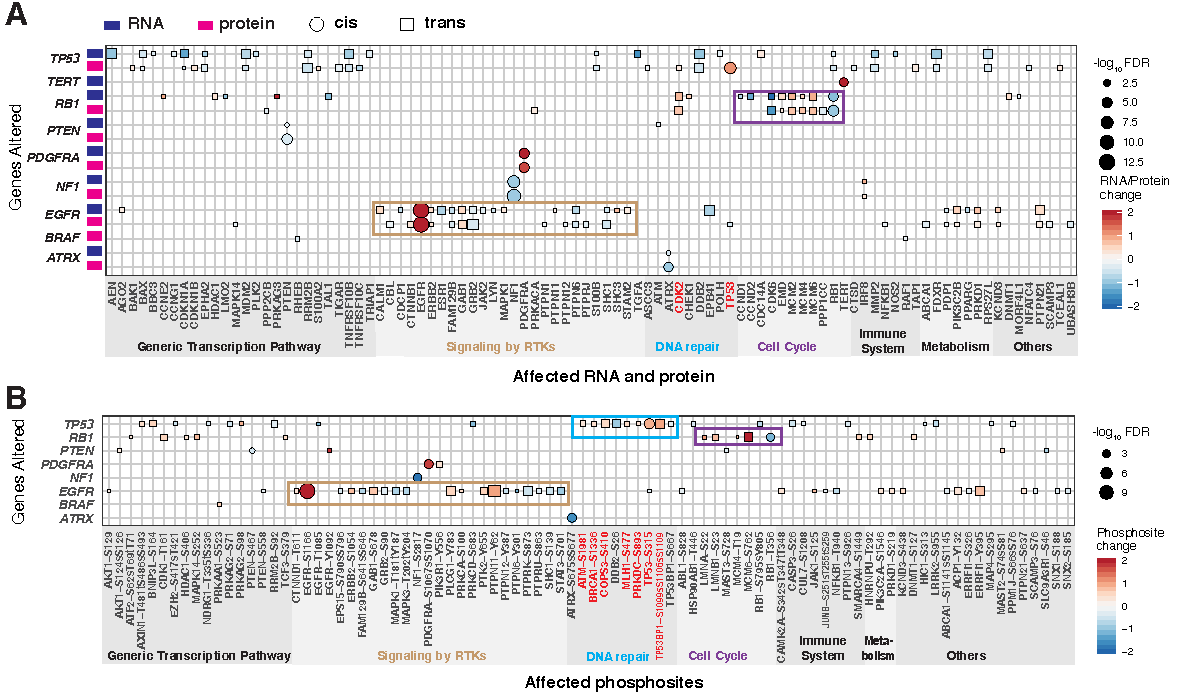
\includegraphics[width=\linewidth]{figures/chap04_cptac_gbm_discov/figure2_mut_impact.pdf}
    \caption[\textit{Cis} and \textit{trans} effects of SMGs on RNA, protein, and phosphorylation abundance.]{%
        \textit{Cis} and \textit{trans} effects of SMGs on protein and phosphorylation.
        \subref{fig:gbm-mut-impact-rna-protein}
        \textit{Cis} and \textit{trans} effects of significantly mutated genes (y axis) on RNA and protein level (x axis) showing that effects are often similar.
        \subref{fig:gbm-mut-impact-phospho}
        \textit{Cis} and \textit{trans} effects of significantly mutated genes (y axis) on protein phosphorylation status (x axis).
    }
    \label{fig:gbm-mut-impact}
\end{figure}

Tumor suppressors \gene{RB1}, \gene{NF1}, \gene{PTEN}, and \gene{ATRX} demonstrated good concordance between genetic alterations and decreased RNA, protein, and phosphorylation levels of their respective gene products. Although the general effect of \gene{TP53} mutations on increased protein stability is known, we identified specific phosphosites that correlate with increased stability. Phosphorylation of TP53 at S315 and TP53BP1 at S1099, S1106, and S1109 correlated with increased TP53 protein expression (Pearson r = 0.89 and 0.53, respectively) (\fref{fig:gbm-mut-impact-rna-protein}, \ref{fig:gbm-mut-impact-phospho}).

We assessed kinases known to phosphorylate TP53 and its downstream targets. In TP53 mutants (\fref{fig:gbm-mut-impact-rna-protein}, \ref{fig:gbm-mut-impact-phospho}), we detected elevated protein and/or phosphorylation in ATR, MAPK3, CDK2, and CDK9, while MDM2 was decreased at both RNA and protein levels. Tumors with \gene{TP53} mutations showed upregulated phosphosites, but not increased protein levels, of DNA repair genes, suggesting specific phosphosite regulation. We observed negative feedback between RB1 and downstream targets, CDK2, CDK6, MCM2, MCM4, and MCM6, while NF1 had similar effects on IRF8 (\fref{fig:gbm-mut-impact-rna-protein}, \ref{fig:gbm-mut-impact-phospho}). \gene{RB1}-altered samples (12\% of the cohort) showed significantly downregulated RB1 and upregulated MCM2, MCM4, and MCM6 protein expression. In addition, in samples with \gene{NF1} alterations, we observed upregulation of protein and RNA of IRF8, a transcription factor that controls microglial motility \cite{masudat_inouek:IRF8Transcriptional2014} (\fref{fig:gbm-mut-impact-rna-protein}, \ref{fig:gbm-mut-impact-phospho}).


\subsection{RTK signaling cascades are activated in GBM}
% TODO: simplify me
Genomic loci associated with RTKs, such as EGFR, PDGFRA, and MET, are frequently amplified in GBM \cite{brennancw_chinl:GBM2013}. We identified 45 tumors with \gene{EGFR} SVs, all having copy number amplifications, suggesting high concordance between SV and CNV (\fref{fig:gbm-overview-mut-landscape}). All tumors with mutated \gene{EGFR} and SV have correspondingly high RNA, protein, and Y1172 phosphorylation levels, indicating EGFR pathway activation. We did not find expression differences between samples having a sole SV event versus those with dual mutation and SV events, suggesting EGFR upregulation in GBM is largely due to SV, as associated with CNV amplification, rather than mutationally driven, which is different from other tumor types, such as lung cancer \cite{tcga:LUAD2014}. We also found nine samples in which \gene{EGFR} SV co-occurred with \gene{PDGFRA} or \gene{FGFR3} SV, while 13 samples with either \gene{PDGFRA} or \gene{FGFR3} alteration did not show any alterations in \gene{EGFR}. For \gene{PDGFRA}, two out of three mutations overlap with SV events. Only one sample with mutation in \gene{PDGFRA} had high PDGFRA RNA and protein expression. For EGFR, n = 53 (WT), 29 (SV), and 16 (SV and MUT); for \gene{PDGFRA}, n = 84 (WT), 12 (SV), and 2 (SV and MUT).

\begin{figure}[tb]
    \centering
    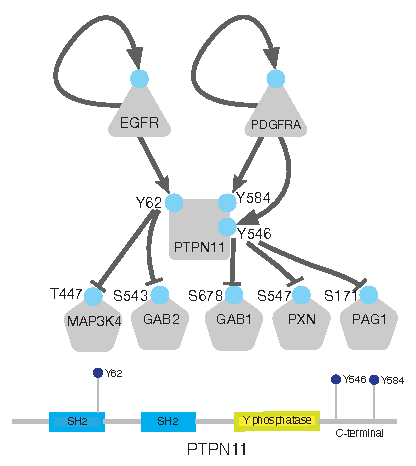
\includegraphics[width=0.5\linewidth]{figures/chap04_cptac_gbm_discov/figure3_ptpn11.pdf}
    \caption[Alterations in RTKs and associations with expression, phosphosite status, and downstream targets.]{%
        Alterations in RTKs and associations with expression, phosphosite status, and downstream targets. The schematic shows dual regulation of PTPN11 by EGFR and PDGFRA and the downstream substrates that PTPN11 may dephosphorylate.
    }
    \label{fig:gbm-ptpn11}
\end{figure}

We also observed increased phosphorylation levels of PTPN11-Y62, PLCG1-Y783, RB1-S795Y805, MAP3K1-S1408, and specific EGFR sites in \gene{EGFR}-altered samples. Notably, the total protein level of PTPN11 was comparable between the two groups, suggesting its activity is regulated primarily by phosphorylation. A similar pattern is observed with PLCG1 (PLCγ1), where Y783 phosphorylation was significantly higher in \gene{EGFR}-altered versus \gene{EGFR}-WT samples (Wilcox false discovery rate [FDR] < 0.01; \fref{fig:gbm-rtk-ihc-plcg1-gab}), despite no significant difference in PLCγ1 protein expression (FDR = 0.11). Since phosphorylation of PLCG1 on Y783 is activating \cite{poulinb_rheesg:IntramolecularInteraction2005}, this could provide a mechanism for EGFR activation of PLCG1’s known effects on proliferation, migration, and invasiveness \cite{kunzek_brauningera:RecurrentActivating2014}.

\begin{figure}[p]
    \centering
    \phantomlabel{fig:gbm-rtk-ihc-alter-impact}
    \phantomlabel{fig:gbm-rtk-ihc-fgfr3-fusion}
    \phantomlabel{fig:gbm-rtk-ihc-plcg1-gab}
    \phantomlabel{fig:gbm-rtk-ihc-ihc-sox9-gab1}
    \phantomlabel{fig:gbm-rtk-ihc-ihc-im1-im4}
    \phantomlabel{fig:gbm-rtk-ihc-ihc-all-ims}
    \includegraphics[height=0.93\textheight]{figures/chap04_cptac_gbm_discov/figures4_validation.pdf}
    \caption[RNA, protein and phosphosite level change in samples with different RTK alterations, and IHC validations.]{%
        RNA, protein and phosphosite level change in samples with different RTK alterations, and IHC validations.
        \legendcontdnote
    }
    \label{fig:gbm-rtk-ihc}
\end{figure}
\begin{figure}[t]
    \centering
    \legend{%
        \legendcontdref{fig:gbm-rtk-ihc}
        \subref{fig:gbm-rtk-ihc-alter-impact}
        The comparison of CNV, RNA and protein expressions and phosphosite level between EGFR altered and WT samples (left panel) and PDGFRA altered and WT samples (right panel).
        \subref{fig:gbm-rtk-ihc-fgfr3-fusion}
        The comparison of RNA and protein expression of FGFR3 and TACC3 between samples with and without FGFR3-TACC3 fusion and the breakpoints found in FGFR3 from RNA-Seq data (n = 94 and 5, respectively). Five samples with FGFR3-TACC3 fusions with an intact FGFR3 kinase domain. Three samples which are protein expression outliers in FGFR3 are marked by larger circles.
        \subref{fig:gbm-rtk-ihc-plcg1-gab}
        The comparison of PLCG1, GAB1, and GRB2 protein expression and PLCG1-Y783 phosphosite level between EGFR altered (n = 46) and WT (n = 53) samples.
        \subref{fig:gbm-rtk-ihc-ihc-sox9-gab1}
        Immunohistochemistry staining for SOX9 and GAB1 expression in EGFR altered and WT tumors is concordant with the mass spectrometry findings. Positive IDH1 R132H staining of the ATRX WT and IDH1 mutant tumor. Scale bars: 100 μm.
        \subref{fig:gbm-rtk-ihc-ihc-im1-im4}
        Immunohistochemistry staining for CD68, CD163, CD3, PD-1, PD-L1 in tumors of different immune subtypes is concordant with the mass spectrometry and gene expression analyses. Scale bars: 100 μm.
        \subref{fig:gbm-rtk-ihc-ihc-all-ims}
        Immunohistochemistry staining for CD68 and CD3 in tumors of all four immune subtypes is concordant with the mass spectrometry and gene expression analyses. Scale bars: 100 μm.
    }
\end{figure}

We performed a kinase-substrate study for EGFR and PDGFRA and identified high levels of GAB1 phosphorylation at Y689 and Y657, consistent with high EGFR expression. In addition, PTPN11 phosphosites at Y546 and Y584 were associated with high PDGFRA expression (\fref{fig:gbm-ptpn11}) and have been observed in lung cancers with ALK fusions \cite{voenac_chiarler:TyrosinePhosphatase2007}. Activation of PTPN11 through either EGFR- or PDGFRA-related phosphorylation in GBM suggests it may represent a shared RTK signaling hub. PTPN11, GAB1, and GRB2 form a complex and are co-regulated by RTKs to activate the RAS pathway \cite{montagnera_raynalp:NovelRole2005}. Figures \ref{fig:gbm-mut-impact-rna-protein} and \ref{fig:gbm-rtk-ihc-plcg1-gab} show that EGFR activation status is associated with upregulated GAB1 and downregulated GRB2 protein expression. We validated the elevated GAB1 expression in EGFR-altered tumors using IHC (\fref{fig:gbm-rtk-ihc-ihc-sox9-gab1}).


\subsection{Distinct immune marker expression and epigenetic events characterize GBM immune subtypes}



\section{Discussion}

\chapter{Conclusion and Future Directions}
\label{chap:conclusion}
% Discussion: remaining challenges, the benefits in another fields than oncology


\begin{figure}[tb]
    \centering
    \includegraphics[width=0.6\linewidth]{figures/chap05_conclusion/cptac_gbm_cancer_cell_cover.png}
    \caption[Better disease understanding through a lens for an integrative view of multi-omics datasets.]{Better disease understanding through a lens for an integrative view of multi-omics datasets. Cover art of \textit{Cancer Cell} (April 2021 issue). Artwork by Jessica Johnson \url{https://jessicajohnsonart.com/}.}
    \label{fig:lens-multi-omics}
\end{figure}


\begin{SingleSpace}
\printbibliography
\end{SingleSpace}

\appendix
% \chapter{Open Source Tool and Pipeline Development}
\label{app:oss-pipeline-dev}


\end{document}
